\documentclass{beamer-control}
\usepackage{beamer-control-singlefile}
\INCLUDEONLY{Laplace Transforms}
\begin{document}
\CONCEPT{Laplace Transforms}

\begin{SUMMARY}
\begin{itemize}
\item Why the Laplace transform is a useful tool
\item Brief mathematical description of the Laplace transform
\item Example of solving an ODE
\item Two `theorems' which provide simple useful properties
\end{itemize}
\vfill References:
\begin{itemize}
\item \astrom{Section 9.3 `Laplace Transforms`}
\end{itemize}
\end{SUMMARY}



\begin{frame}{Reminder from TFs}
  \begin{itemize}
    \item Recall we previously analysed ODEs using a solution involving $\ee^{st}$
    \item What is $s$? Call it `complex frequency'
    \item For $s=\jj\ww$ we have sinusoidal signals with frequency $\ww$\\
          (recall $\ee^{\jj\ww t}=\cos(\ww t)+\ii \sin(\ww t)$)
    \item When we introduce a real term ($s=\sigma+\jj\ww$) this includes exponential decay (or growth)
    \item \alert{We can analyse linear systems as functions of $s$ instead of $t$}
    \item Why? Allows recipes for analytical solutions of ODEs 
  \end{itemize}
\end{frame}


\begin{frame}{Mathematical foundation}
  Close relationship between:
  \begin{itemize}
  \item Fourier series -- representing periodic signals as infinite sums of sinusoids (each with differing frequencies and amplitudes)
  \item Fourier/Laplace transforms -- converting ODEs analytically into the frequency domain 
  \item Discrete Fourier Transforms (or FFTs) -- taking measured data and numerically calculating the frequency response
  \end{itemize}
\end{frame}

\SUBCONCEPT{The Laplace transform}

\begin{frame}{Mathematically}
  Laplace transform for $s\in\mathbb{C}$:\footnote{N.B. some variances in how the limits are defined, not important here.}
  \begin{gather}
  \mathcal{L}\{f(t)\} = F(s) = \int_0^\infty f(t) e^{-st} dt
  \end{gather}
  Fourier transform for $s=\ii\omega$, with $\omega\in\mathbb{R}$:
  \begin{gather}
  \mathcal{F}\{f(t)\} = F(\omega) = \int_{-\infty}^\infty f(t) e^{-\ii\omega t} dt
  \end{gather}
  These are linear transforms:
  \begin{gather}
  \mathcal{L}\{\alert{c} f(t)\} = \alert{c}\mathcal{L}\{f(t)\} \\
  \mathcal{L}\alert{\bigl\{}f(t)\alert{+}g(t)\alert{\bigr\}} = \mathcal{L}\{f(t)\}\alert{+}\mathcal{L}\{g(t)\}
  \end{gather}
\end{frame}


\begin{frame}{This is not a course about transforms}
  Need to know (memorise):
  \begin{align}
  s &= \sigma+\jj\ww \qquad (\jj^2=-1) \\
  \mathcal{L}\bigl\{f(t)\bigr\} &= F(s) \\
  \mathcal{L}\bigl\{\frac{d}{dt}f(t)\bigr\} &= sF(s)  \\
  \mathcal{L}\bigr\{\int f(t)dt\bigr\} &= \frac{1}{s}F(s)
  \end{align}
  Note, in control, we always linearise our systems around an equilibrium and can therefore ignore initial conditions $f(0)$
\end{frame}

\begin{frame}
\frametitle{Mass-spring-damper transfer function example}
\begin{gather}
m \ddot x(t) + c \dot x(t) + kx = f(t) \\
m s^2 X(s) + c s X(s) + k X(s) = F(s) \\
\frac{X(s)}{F(s)} = \frac{1}{ms^2+cs+k}
\end{gather}
For $m=1$, $c=6$, $k=5$:
  \begin{gather}
\frac{X(s)}{F(s)} = \frac{1}{s^2+6s+5} = \frac{1}{(s+1)(s+5)}
  \end{gather}
Here we have `real poles' $s=-1, -5$: these govern the behaviour of the solution
\end{frame}

\begin{frame}
\frametitle{Tables of Laplace transforms}
  \centering
  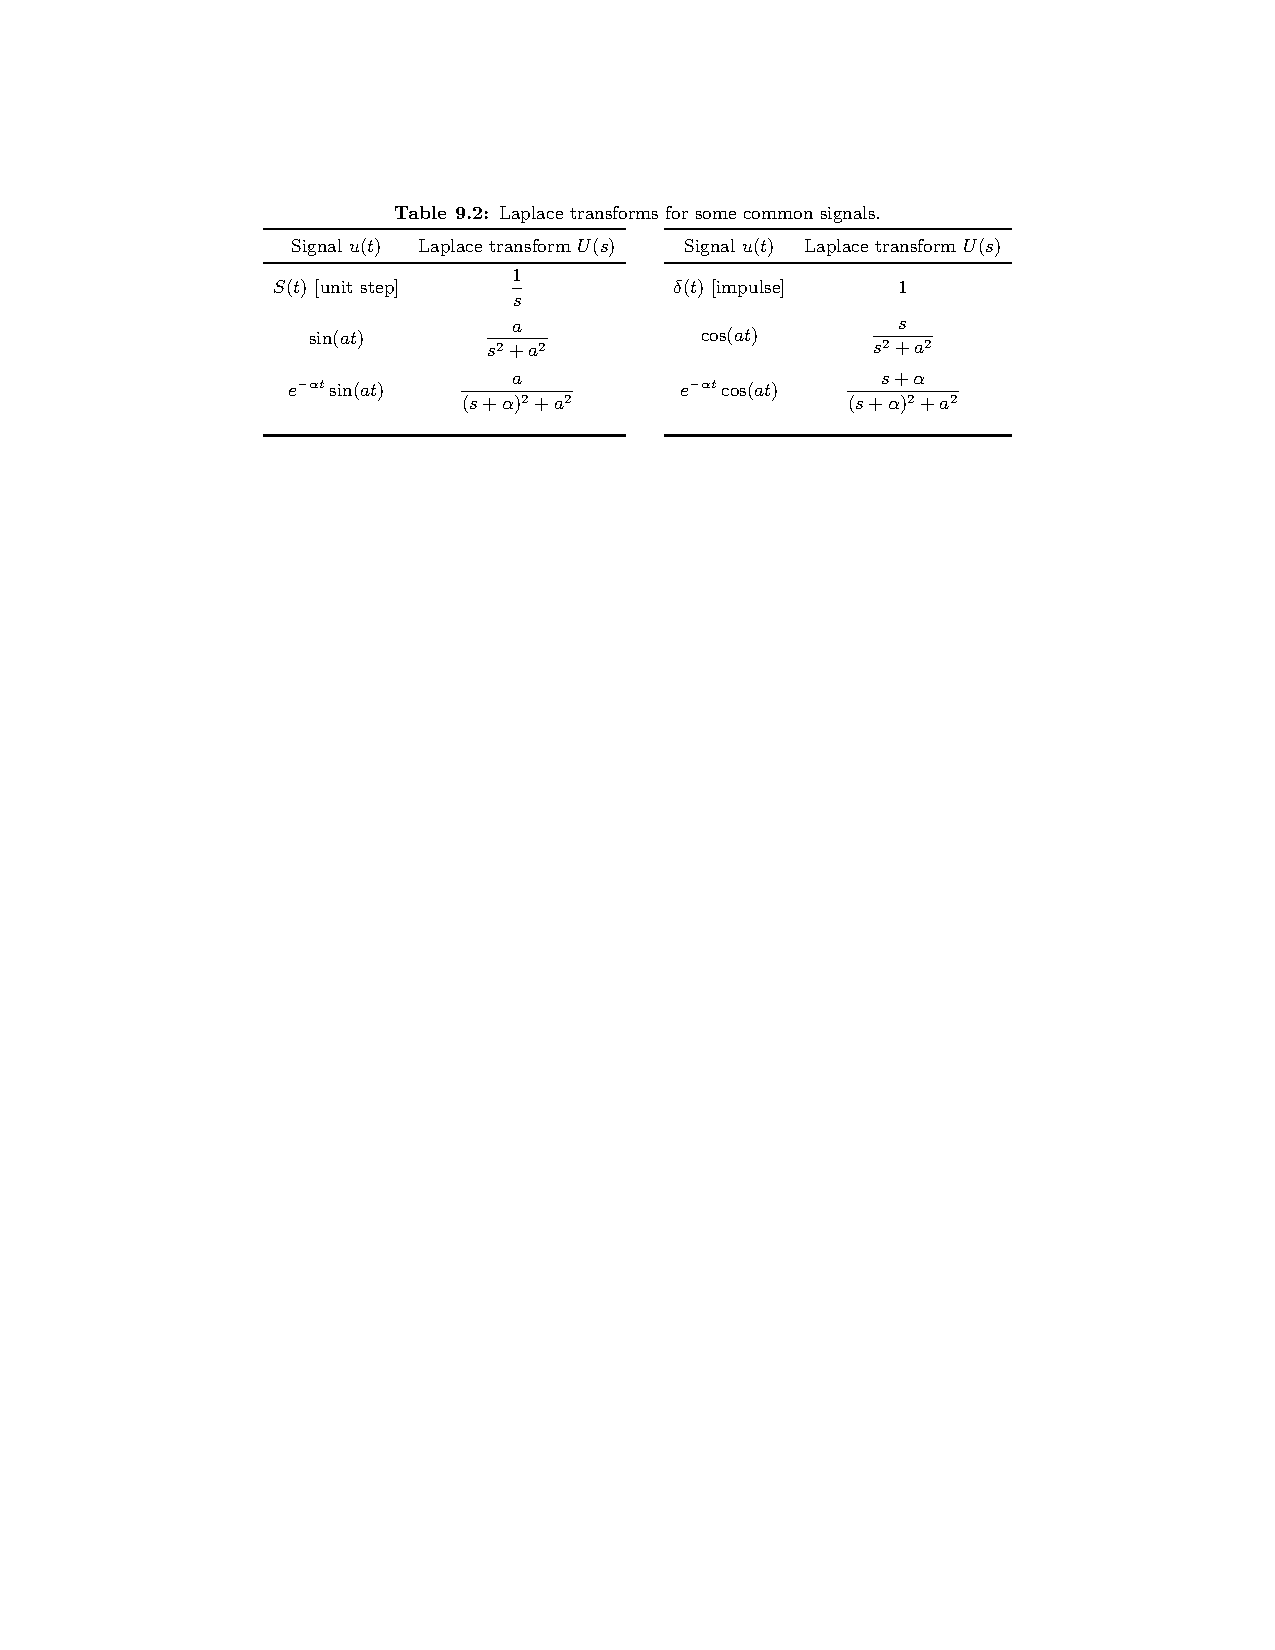
\includegraphics[width=\linewidth]{table9.2-laplace-transforms}
\end{frame}

\begin{frame}
\frametitle{Inverse Laplace transforms}
  \begin{gather}
    f(t) = \mathcal{L}^{-1}\bigl\{F(s)\bigr\} \\
    \mathcal{L}^{-1}\bigl\{b F(s) + c G(s)\bigr\} = b\mathcal{L}^{-1}\bigl\{F(s)\bigr\} + c\mathcal{L}^{-1}\bigl\{G(s)\bigr\}
  \end{gather}
  $\therefore$ A transfer function $P(s)/Q(s)$ with rational polynomials is solved using factorisation and partial fraction expansion and the result is a sum of exponential and/or sinusoid terms, e.g.:
  \begin{gather}
    \mathcal{L}^{-1}\left\{ \frac{3s+8}{s^2+2s+5} \right\} = \ee^{-t} \left( 3\cos 2t + \tfrac{5}{2}\sin 2t \right)
  \end{gather}
\end{frame}

\begin{frame}
\frametitle{Generalised second order step input example}

\begin{gather}
U(s) G(s) = \frac{1}{s}\frac{K\omega_n^2}{s^2+2\zeta\omega_ns+\omega_n^2}
\end{gather}
Assume $\zz<1$:
\begin{align}
x(t) &= \Lapl^{-1}\left\{ \frac{1}{s}\frac{K\wn^2}{s^2+2\zz\wn s+\wn^2} \right\} \\
\intertext{\em using tables of inverse Laplace transforms:}
x(t) &= K - K\frac{\exp(-\zz\wn t)}{\sqrt{1-\zz^2}}\sin\left[\wn t\sqrt{1-\zz^2}+\arccos\zz\right] \label{eq:xt2o}
\end{align}
(Now differentiate \& solve for $x'(t)=0$ to find peak response.)

\end{frame}

\SUBCONCEPT{Initial and final value theorems}

\begin{frame}
\frametitle{Initial value theorem}

\begin{gather}
\lim_{t\to0} f(t) = \lim_{s\to\infty} s F(s)
\end{gather}
Often used for transfer functions with step inputs. E.g. for system $G(s)$, step input $R(s)$, and output $U(s)$:
\begin{gather}
R(s) = \frac{1}{s} \qquad\text{\AMref{Table 9.2}}\\
u(0) = \lim_{t\to0} u(t) = \lim_{s\to\infty} s U(s) = \lim_{s\to\infty} s R(s)G(s) \\
u(0) = G(\infty)
\end{gather}
\end{frame}

\begin{frame}
\frametitle{Initial value theorem example}

Mass-spring-damper:
\begin{gather}
\frac{X(s)}{F(s)} = \frac{1}{ms^2+cs+k} \\
x(t)|_{t=0} = \lim_{s\to\infty} \frac{1}{ms^2+cs+k} = 0
\end{gather}
What does this mean? After a constant force, the response starts from zero and then builds up.

\bigskip
\QUIZ{What is the initial response to an impulse?}
\end{frame}

\begin{frame}
\frametitle{Final value theorem}

\begin{gather}
\lim_{t\to\infty} f(t) = \lim_{s\to0} s F(s)
\end{gather}
Again, very helpful when analysing step inputs. For system $G(s)$, step input $R(s)$, and output $U(s)$:
\begin{gather}
R(s) = \frac{1}{s} \qquad\text{\AMref{Table 9.2}}\\
u(\infty) = \lim_{t\to\infty} u(t) = \lim_{s\to0} s U(s) = \lim_{s\to0} s R(s)G(s) \\
u(\infty) = G(0)
\end{gather}
\end{frame}

\begin{frame}
\frametitle{Final value theorem example}

Mass-spring-damper:
\begin{gather}
\frac{X(s)}{F(s)} = \frac{1}{ms^2+cs+k} \\
x(t)|_{t=\infty} = \lim_{s\to0} \frac{1}{ms^2+cs+k} = \frac{1}{k}
\end{gather}
What does this mean? After a constant force is applied, the response starts from zero and settles to a certain value ($\frac{1}{k}$).

\bigskip
\QUIZ{What is the final response to an impulse?}
\end{frame}

\begin{frame}
\frametitle{Generalised second order system}
Recall \eqref{xt2o}:
\begin{align}
U(s)G(s) & = \frac{1}{s}\frac{K\omega_n^2}{s^2+2\zeta\omega_ns+\omega_n^2} \\
x(t) &= K - K\frac{\exp(-\zz\wn t)}{\sqrt{1-\zz^2}}\sin\left[\wn t\sqrt{1-\zz^2}+\arccos\zz\right]
\end{align}
Note:
\begin{align}
\underbrace{G(s)|_{s=0}}_{\text{DC gain}} &= K & \underbrace{x(t)|_{t\to \infty}}_{\text{SS resp.}} &= K
\end{align}
DC gain of the plant = steady state response to a step
\end{frame}

\SUMMARYFRAME
\FINALE

\end{document}
